\documentclass{sig-alternate}

\usepackage{amsmath}
\usepackage{graphicx}
\usepackage{subfigure}
\usepackage{color}
\usepackage{xspace}
\usepackage{url}
 \usepackage[utf8]{inputenc}

 % lorem
\newcommand{\lorem}               {\textcolor{green}{Lorem ipsum dolor sit amet, consectetur adipisicing elit, sed do eiusmod tempor incididunt ut labore et dolore magna aliqua. Ut enim ad minim veniam, quis nostrud exercitation ullamco laboris nisi ut aliquip ex ea commodo consequat. Duis aute irure dolor in reprehenderit in voluptate velit esse cillum dolore eu fugiat nulla pariatur. Excepteur sint occaecat cupidatat non proident, sunt in culpa qui officia deserunt mollit anim id est laborum.}}

% reviews
\newcommand{\thomas}[1]             {\textcolor{blue}{[Thomas] #1}}
\newcommand{\keoma}[1]              {\textcolor{green}{[Keoma] #1}}
\newcommand{\remy}[1]               {\textcolor{yellow}{[Remy] #1}}
\newcommand{\jonathan}[1]           {\textcolor{pink}{[Jonathan] #1}}

% shortcuts
\newcommand{\name}                  {PEACH\xspace}
\newcommand{\smip}                  {SmartMesh~IP\xspace}

\graphicspath{{figures/}}

\begin{document}
\title{Feedbacks from a real-world low-power wireless sensor network deployment}

\numberofauthors{3}
\author{
  \alignauthor Brun-Laguna Keoma\\
    \affaddr{Inria, EVA team, Paris, France}\\
    \email{keoma.brun@inria.fr}
  \alignauthor Rémy Léone\\
    \affaddr{Inria, EVA team, Paris, France}\\
    \email{remy.leone@inria.fr}
  \alignauthor Jonathan Muñoz\\
    \affaddr{Inria, EVA team, Paris, France}\\
    \affaddr{Gridbee, France}\\
    \email{jonathan.munoz@inria.fr}
}

\maketitle

\begin{abstract}
\lorem
\end{abstract}


%==============================================================================
\section{Introduction}
\label{sec:intro}

% the PEACH project

In April 2016, three research teams from different countries joined to start the deployment of a frost events prediction system~\cite{watteyne16peach}.
The goal of this project is to be able to precisely predict frost events and consequently reduce the impact of frost on peach production.
Low temperatures have a very harmful impact on peach production as in 2013, 85\% of the production in the Mendoza region (western Argentina) was lost because of frost.
Frost detection systems already exist but few actually able to propose prediction.

% the architecture

The deployed solution is composed of a low-power wireless network and a back-end system to retrieve and visualize the data.
The network is formed by \smip devices from the Linear Technology company and is in charge of measuring the orchard environment, gather the data into a gateway and pass it to the back-end system.
Both sensor values and network statistics are collected.
The back-end system stores and backups the data and provide both a visual interface and an API to access the data minutes after it was measured in Argentina.

% the deployment

The low-power wireless network is composed of 21 nodes uniformly distributed between the peach trees.
The covered area is an orchard with 204 trees on a 50*100m surface.
Each network mote is placed inside a water-tight box that is fixed on a 4m pole~\ref{fig:orchard}.
Because the project is on its first stage, we only measure air temperature from built-in sensors.
During the second stage, we will introduce additional sensors such as air temperature at different high, air relative humidity, soil moisture and soil temperature.

\begin{figure}
    \centering
    \includegraphics[width=\columnwidth]{orchard}
    \caption{The wireless motes deployed inside the orchard in Mendoza (Argentina)}
    \label{fig:orchard}
\end{figure}

% the data

Each mote produce a temperature value every 30 seconds and network statistics, called ``health-reports'', every 5~minutes.
In 3~months, we gathered more than 2M~temperature value, and more than 180K~network statistics.
The health reports produced by any mote contain information about the mote itself and also about its neighbors.
%65184 HR_DEVICE, 63245 HR_DISCOVERED and 50285 HR_NEIGHBORS


\lorem

% the goal of this paper

The goal of this paper is to present the first feedbacks we have from the 3-month-old project.
\lorem

% paper organisation
This paper is organized as follow:
Section~\ref{sec:collected} gives an in-depth description of the data we collect.

\lorem

%==============================================================================
\section{Collected Data}
\label{sec:collected}

% health report description

\lorem

% HR_DEVICE

\lorem

% HR_DISCOVERED

\lorem

% HR_NEIGHBORS

\lorem

%==============================================================================
\section{RSSI}
\label{sec:rssi}

% RSSI expectations

\lorem

% what we found

\lorem

% periodic RSSI

\begin{figure}
    \centering
    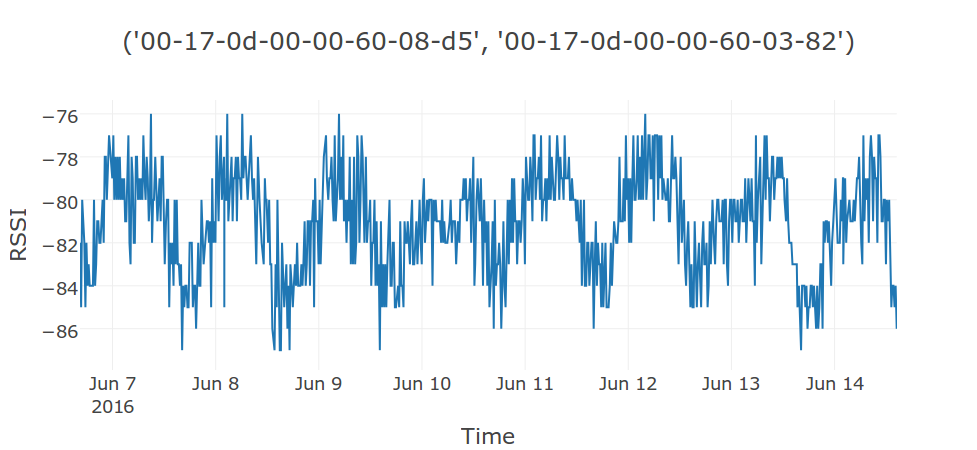
\includegraphics[width=\columnwidth]{periodic_rssi}
    \caption{The RSSI value of node 0f-66 as received by mote 03-82 over a week.}
    \label{fig:periodic_rssi}
\end{figure}


%==============================================================================
\section{Topology}
\label{sec:topology}

% topology expectations

\lorem

% what we found

\lorem

%==============================================================================
\section{Reliability}
\label{sec:reliability}

% reliability expectation

\lorem

%==============================================================================
\section{Technology Feedbacks}
\label{sec:technology}

% intro (why is this section relevant)

\lorem

% SOL

\lorem

% database

\lorem

% grafana

\lorem

% conclusion


%==============================================================================

\bibliographystyle{abbrv}
\bibliography{16chants}

\end{document}

%
